\documentclass[preprint,12pt,authoryear]{elsarticle}
\usepackage[T1]{fontenc}
\usepackage{amsmath,amssymb}
\usepackage{graphicx}
\graphicspath{{figures/}}
\usepackage{booktabs}
\usepackage[colorlinks,citecolor=black,linkcolor=black,urlcolor=blue]{hyperref}
\journal{Finance Research Letters}

\begin{document}
\begin{frontmatter}

\title{Synchronized speculative positioning in futures markets:\\
a pre-registered null and exploratory sub-market effects}

\author{Arjun Kathiravelu}
\ead{arjun.kathiravelu@etu.unige.ch}
\address{University of Geneva, Geneva, Switzerland}

\begin{abstract}
Coupled-oscillator (Kuramoto) measures are proposed as crowding indicators:
when traders' position cycles align, synchronized exits should follow. We
test this on CFTC leveraged-fund and managed-money positions in 32 futures
markets with a causal phase and a pre-registered design. Pooled, the order
parameter predicts neither returns, drawdowns nor volatility of the
speculative book, in or out of sample, and its excess over independence is
89\% ordinary comovement of positions. Exploratory splits tell a different
story: in currencies, synchronization precedes deeper drawdowns of the
leveraged-fund book beyond aggregate positioning ($-0.24$ s.d., out-of-sample
$R^2$ of 6.8\%), while in commodities it precedes continuation. We register
held-out tests of both.
\end{abstract}

\begin{keyword}
crowding \sep synchronization \sep Kuramoto model \sep Commitments of Traders
\sep currency crash risk \sep pre-registration
\JEL G11 \sep G13 \sep G14 \sep G17
\end{keyword}
\end{frontmatter}

\noindent\textit{Note on this version.} This paper replaces the version posted
on SSRN in March 2026 under the title ``Endogenous Kuramoto Synchronization in
Algorithmic Trading Flows''. The empirical results of that version are
withdrawn; \ref{app:withdrawn} lists them with the reason for each.

\section{Introduction}

Crowded positions unwind together \citep{Pedersen2009,Stein2009,KhandaniLo2011}.
Measures of crowding infer it from holdings, from return comovement
\citep{LouPolk2022}, or from futures positioning, which also carries hedging
pressure \citep{Bessembinder1992,deRoon2000,KangRouwenhorstTang2020}. In
currencies, speculative net positions predict crash risk
\citep{BrunnermeierNagelPedersen2008}. Synchronization models from physics add
a different object: map each trader group to a phase oscillator and measure
alignment with the Kuramoto order parameter
$r(t) = |N^{-1}\sum_i e^{i\theta_i(t)}|$ \citep{Strogatz2000,Acebron2005}.
High $r$ is read as crowding.

This letter tests that reading on real positions. An earlier, unpublished
version of this framework built phases from synthetic strategies with an
event-anchored phase that interpolated to the next flow peak, hence used
future data, and estimated a liquidity elasticity from a Corwin--Schultz
spread, which is itself a function of the high--low range
(\ref{app:earlier}). We replace both with a causal phase on CFTC
positions, pre-register the test, and report everything that followed:
a registered null, a review that exposed why it is null, the exploratory
sub-market effects behind it, and a registered held-out test of those
effects.

\section{Data and registered design}
\label{sec:design}

Positions are the weekly CFTC Commitments of Traders, futures only, Tuesday
as-of: leveraged funds in the Traders in Financial Futures report (equity
indices, Treasuries, currencies) and managed money in the disaggregated
report (energy, metals, grains, livestock). The net position of market $i$ is
$x_i(t) = (\text{long} - \text{short})/\text{open interest}$. Archives were
downloaded on 7 November 2026; histories before 2009--2010 are CFTC back-casts.
A report enters from the first trading day on or after the Monday following
its as-of date (it is released on Friday), and report weeks around the 2013,
2018--19 and 2025 shutdowns are excluded. Prices are back-adjusted daily
futures; returns are daily price changes scaled by trailing volatility. The
universe is every market with at least 85\% coverage of both the CFTC series
(2009--2026) and our price files (2010--2026): 32 markets. The price
requirement removes the softs, palladium and KC wheat.

The phase is causal: with $z_i(t)$ the 156-week trailing z-score of $x_i$ and
$d_i(t)$ the weekly change of $x_i$ divided by the trailing standard deviation
of changes, $\theta_i(t) = \operatorname{atan2}(-d_i, z_i)$, so that 0 is a
maximal long and $\pi$ a maximal short. Every phase at $t$ is unchanged when
data after $t$ are altered (tested).

The registered hypotheses were: H1, mean $r$ exceeds a null that circularly
shifts each market's phase series ($p<0.01$); H2, $r$ predicts at least one of
the 4-week return (Y1), maximum drawdown (Y2) or volatility ratio (Y3) of the
speculative book (each market long or short with the sign of $x_i$,
volatility-scaled, equal weight), with controls for the book's trailing
return, trailing volatility ratio, pairwise correlation and first-component
share of position changes, and mean $|z_i|$; stationary block bootstrap
\citep{PolitisRomano1994} and Romano--Wolf adjustment \citep{RomanoWolf2005};
H3, out-of-sample improvement over the model without $r$ \citep{ClarkWest2007},
training to 2017 and testing on 2018--2026. A full crowding paper required all
three. The registration (\texttt{PREREG.md}) and code were committed before
each run; these timestamps are self-reported, not an external registration.
A first run, affected by a loading bug, used only the 16 commodity markets; it
is kept and reported in the package.

\section{Registered results}

\begin{figure}[t]
\centering
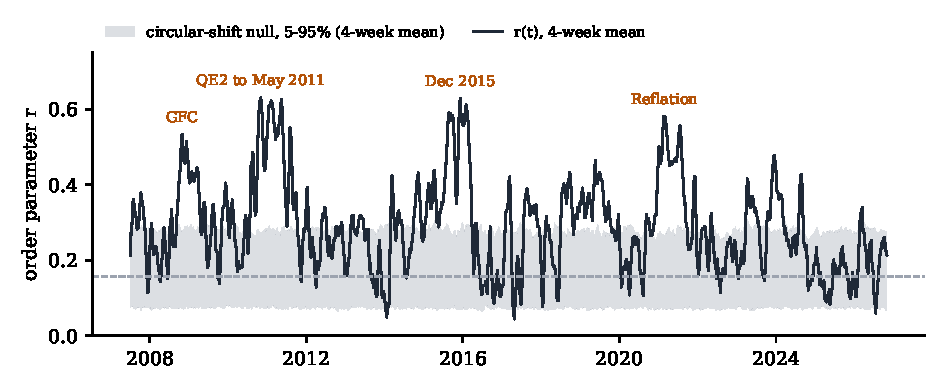
\includegraphics[width=\textwidth]{fig_r_real.pdf}
\caption{Order parameter of speculative positioning across 32 futures markets
(causal phase, 4-week mean) against the pointwise 5--95\% band of 500
circular-shift surrogates. Under the null about 5\% of weeks exceed the band.}
\label{fig:r}
\end{figure}

H1 holds as registered: mean $r$ is 0.287 against a surrogate mean of 0.156
($p=0.0005$, the smallest attainable with 2{,}000 surrogates), equal to the
independence floor $\sqrt{\pi/4N}=0.157$ (Figure~\ref{fig:r}). H2 and H3 fail
(Table~\ref{tab:h2}): no outcome has an adjusted $p$ below 0.33, and
out-of-sample $R^2$ stays under 1\%. The test could detect effects of about
0.15 s.d.\ of the outcome; for drawdowns the 95\% interval reaches
$-0.20$ s.d., so small crowding effects are not excluded.

\begin{table}[t]
\centering
\caption{Registered predictive tests, 32 markets (770 weeks, entries 2010-08
to 2026-01). $b$: coefficient on $r$ in s.d.\ of the outcome, with Newey--West
95\% interval; $p_{RW}$: Romano--Wolf adjusted; $p_{CW}$: Clark--West
one-sided, 396 test weeks; MDE: minimum detectable effect, 80\% power.}
\label{tab:h2}
\small
\begin{tabular}{lrrrrrr}
\toprule
Outcome & $b$ & 95\% interval & $p_{RW}$ & $p_{CW}$ & $R^2_{oos}$ & MDE \\
\midrule
Y1 return     & $0.04$ & $[-0.07,\ 0.15]$ & 0.78 & 0.40 & 0.000 & 0.16 \\
Y2 drawdown   & $-0.09$ & $[-0.20,\ 0.02]$ & 0.33 & 0.21 & 0.005 & 0.16 \\
Y3 vol.\ ratio & $-0.01$ & $[-0.11,\ 0.09]$ & 0.78 & 0.82 & $-0.006$ & 0.14 \\
\bottomrule
\end{tabular}
\end{table}

\section{Why the pooled test is null (exploratory)}

The analyses in this section were run after the registered results and an
adversarial review; they are hypothesis-generating.

\paragraph{H1 is mostly comovement.} The circular-shift null removes all
dependence between markets, so any common factor rejects it. A multivariate
Fourier surrogate of weekly position changes keeps every cross-correlation
and spectrum and randomizes the rest \citep{PrichardTheiler1994}. Against it,
synchronization is marginal (Table~\ref{tab:ft}): 89\% of the excess of $r$
over independence is linear comovement, as expected when traders respond to
common shocks \citep{TeramaeTanaka2004}. Only commodities keep a clear excess
($p=0.006$). The order parameter is also close to a breadth measure: its rank
correlation with $|N^{-1}\sum_i \operatorname{sign} z_i|$ is 0.80, and phases
reduced to the sign of $z_i$ give a mean $r$ of 0.271 against 0.287.

\begin{table}[t]
\centering
\caption{Mean $r$ against two nulls (500 surrogates each; complete-case
panels, so the observed values differ slightly from the registered one).
Share: part of the excess over the circular-shift mean that the
Fourier null reproduces.}
\label{tab:ft}
\small
\begin{tabular}{lrrrrr}
\toprule
Markets & observed & circular mean & Fourier mean & $p_{\text{Fourier}}$ & share \\
\midrule
All 32 & 0.277 & 0.160 & 0.264 & 0.036 & 0.89 \\
Commodities (16) & 0.368 & 0.225 & 0.342 & 0.006 & 0.82 \\
Financials (16) & 0.306 & 0.233 & 0.298 & 0.194 & 0.89 \\
\quad Currencies (8) & 0.424 & 0.315 & 0.417 & 0.253 & 0.93 \\
\quad Rates and equity (8) & 0.427 & 0.329 & 0.404 & 0.052 & 0.76 \\
\bottomrule
\end{tabular}
\end{table}

\paragraph{The pooled null averages opposite effects.} Table~\ref{tab:sub}
splits the registered H2 and H3. In currencies, higher $r$ precedes deeper
drawdowns of the leveraged-fund book ($-0.26$ s.d., $t=-4.85$), out of sample
as well ($R^2_{oos}=6.8\%$). In commodities, it precedes higher returns of
the managed-money book ($+0.18$ s.d.), consistent with trend continuation
\citep{MoskowitzOoiPedersen2012}. Rates and equity indices show a drawdown
effect too, but there leveraged funds are net short in most weeks in the
longer Treasury contracts and the S\&P~500 contract (UB 100\%, ES 98\%, ZB
84\%, ZF 71\%), positions that partly reflect basis trades and hedges of cash
holdings rather than directional bets \citep{BarthKahn2021}; the effect there
disappears once aggregate positioning is controlled.
With $|N^{-1}\sum_i z_i|$ and $N^{-1}\sum_i z_i$ added, the channel of
\citet{BrunnermeierNagelPedersen2008}, the currency effect stays
($-0.24$ s.d., $t=-3.47$, $p_{RW}=0.001$) and so does commodity continuation
($+0.13$ s.d., $t=2.14$, $p_{RW}=0.034$). Five sub-universes and three
outcomes make 15 tests. With the registered controls both effects survive a
Bonferroni correction across them; with aggregate positioning added, only
the currency effect does.

\begin{table}[t]
\centering
\caption{Exploratory split of the registered tests (registered controls).
Last column: coefficient on $r$ with aggregate positioning
($|N^{-1}\sum z_i|$, $N^{-1}\sum z_i$) added, $t$ in brackets.}
\label{tab:sub}
\small
\begin{tabular}{llrrrrr}
\toprule
Markets & Outcome & $b$ & $t_{NW}$ & $p_{CW}$ & $R^2_{oos}$ & $b$ with positioning \\
\midrule
Currencies (8) & Y2 drawdown & $-0.26$ & $-4.85$ & $<0.001$ & 0.068 & $-0.24$ [$-3.47$] \\
Rates, equity (8) & Y2 drawdown & $-0.28$ & $-3.81$ & $<0.001$ & 0.050 & $-0.13$ [$-1.48$] \\
Commodities (16) & Y1 return & $0.18$ & $3.20$ & 0.020 & 0.026 & $0.13$ [$2.14$] \\
\bottomrule
\end{tabular}
\end{table}

\section{Registered held-out tests}

All the effects above come from data already examined. We therefore register
(\texttt{CONFIRM\_PREREG.md}, to be deposited on OSF before any held-out outcome is computed) three one-sided tests on
outcomes no analysis has looked at, each at $\alpha = 0.05/3$, with the
registered controls plus aggregate positioning: CH1, currency $r$ predicts
deeper drawdowns of the currency book on entries from March 2026 to December
2028 (no price after 24 February 2026 has been loaded); CH2a, commodity $r$
predicts higher returns of a managed-money book on six commodity markets never
used in any outcome analysis (cocoa, cotton, coffee, sugar, KC wheat,
palladium); CH2b, the commodity effect on the time hold-out. The code refuses
to run before the registration is recorded and the time hold-out before
February 2029. Power is limited and stated in advance: 44\% for CH1 at the
in-sample effect and 13\% at half of it, 17--30\% for CH2a.

\section{Conclusion}

Speculative positions across futures markets move together, but most of that
alignment is ordinary comovement, and pooled synchronization is not a crowding
warning. The pooled null hides two opposite effects: synchronized
leveraged-fund currency positioning precedes crash risk beyond the level of
positioning, and synchronized commodity positioning precedes continuation.
Both are exploratory and both are now registered for held-out tests.

\section*{Declaration of competing interest}
The author declares no competing interests.

\section*{Funding}
This research received no specific grant from any funding agency.

\section*{Data availability}
Code, both pre-registrations, every result file and the CFTC download script
are at \url{https://github.com/barj28/kuramoto-positioning-sync}; an archived DOI will follow. CFTC data are public.
Futures prices are licensed (Databento) and not redistributed; the weekly
outcome and control rows are included.

\appendix
\section{Two flaws of the earlier framework}
\label{app:earlier}

\paragraph{Event-anchored phases.} Assigning phase 0 to a buying burst, $\pi$
to the next selling burst and interpolating in between needs the date of the
next burst; peak detection that compares $q_t$ with $q_{t+1}$ adds a one-step
leak. Altering a position series after date $\tau$ changes the interpolated
phases before $\tau$; the causal phase of Section~\ref{sec:design} does not
move.

\paragraph{A spread elasticity built from volatility.} The Corwin--Schultz
spread is a function of the daily high--low range, which scales with
volatility \citep{AbdiRanaldo2017}. Simulating a market whose true spread is
constant (true elasticity zero) and regressing $\log(1/S_t)$ on log
volatility gives elasticities of 0.71 to 0.87, close to the mean of 0.73
that the earlier framework reported across 43 CME futures; with volatility measured over the
21 days before $t$ the estimates are 0.73 to 0.89.

\paragraph{Inference.} The earlier work reported i.i.d.\ $p$-values for
correlations between a persistent $r(t)$ and overlapping 21-day forward
drawdowns. Such $p$-values are known to be far too small
\citep{HansenHodrick1980,Valkanov2003}; all inference here is
dependence-robust.

\section{Claims of the March 2026 version that are withdrawn}
\label{app:withdrawn}

\begin{enumerate}
\item The liquidity-elasticity spectrum across 1{,}543 instruments (1{,}500 US
equities and 43 CME futures, from Corwin--Schultz spreads), its sector
ordering, and the finding that Treasury-bill ETFs are the only sector with a
negative elasticity. With a constant true spread, so a true elasticity of zero,
the estimator returns 0.71 to 0.87 with contemporaneous volatility and 0.73 to
0.89 with the lagged 21-day volatility used for equities
(\ref{app:earlier}). The spectrum is not identified by this estimator.
\item The tick-level elasticities of 43 CME futures ($+1.49$ to $-0.56$) and
the four-regime taxonomy built on them. Replacing contemporaneous realized
volatility by its one-day lag, to remove bid-ask bounce, leaves a rank
correlation of 0.24 with the reported estimates, and 24 of the 43 signs change.
\item The order parameter of 4{,}786 synthetic strategy--instrument positions
and every result built on it: its correlation with forward drawdowns
($\rho = +0.196$), the March 2020 episode, the comparison with a
rolling-correlation benchmark (paired $t = 3.04$) and the per-instrument
cross-validations. The Signed Flux Bursts phase interpolated to the next flow
peak and therefore used future data, the strategies were functions of prices
rather than observed positions, and the drawdown correlations were tested with
i.i.d.\ $p$-values on overlapping horizons.
\item The calibration of the mean-field model ($K_0 = 7.47$, $\gamma = -0.147$,
$\delta = 8.45$): $\gamma < 0$ violates the model's own constraint
$\gamma > 0$, and $\delta = 8.45$ contradicts the square-root impact exponent
of 0.5 that the model assumes.
\item The endogenous coupling $K(r)$ and its consequences (stability regimes,
the ``liquidity black hole'', hysteresis, capacity bounds) are not tested in
this paper and are not maintained.
\end{enumerate}

\begin{thebibliography}{99}
\bibitem[Abdi and Ranaldo(2017)]{AbdiRanaldo2017}
Abdi, F., Ranaldo, A., 2017. A simple estimation of bid-ask spreads from daily close, high, and low prices. Review of Financial Studies 30, 4437--4480.
\bibitem[Acebr\'on et~al.(2005)]{Acebron2005}
Acebr\'on, J.A., Bonilla, L.L., P\'erez Vicente, C.J., Ritort, F., Spigler, R., 2005. The Kuramoto model: a simple paradigm for synchronization phenomena. Reviews of Modern Physics 77, 137--185.
\bibitem[Barth and Kahn(2021)]{BarthKahn2021}
Barth, D., Kahn, R.J., 2021. Hedge funds and the Treasury cash-futures disconnect. Office of Financial Research Working Paper 21-01.
\bibitem[Bessembinder(1992)]{Bessembinder1992}
Bessembinder, H., 1992. Systematic risk, hedging pressure, and risk premiums in futures markets. Review of Financial Studies 5, 637--667.
\bibitem[Brunnermeier et~al.(2008)]{BrunnermeierNagelPedersen2008}
Brunnermeier, M.K., Nagel, S., Pedersen, L.H., 2008. Carry trades and currency crashes. NBER Macroeconomics Annual 23, 313--347.
\bibitem[Clark and West(2007)]{ClarkWest2007}
Clark, T.E., West, K.D., 2007. Approximately normal tests for equal predictive accuracy in nested models. Journal of Econometrics 138, 291--311.
\bibitem[de~Roon et~al.(2000)]{deRoon2000}
de Roon, F.A., Nijman, T.E., Veld, C., 2000. Hedging pressure effects in futures markets. Journal of Finance 55, 1437--1456.
\bibitem[Hansen and Hodrick(1980)]{HansenHodrick1980}
Hansen, L.P., Hodrick, R.J., 1980. Forward exchange rates as optimal predictors of future spot rates: an econometric analysis. Journal of Political Economy 88, 829--853.
\bibitem[Kang et~al.(2020)]{KangRouwenhorstTang2020}
Kang, W., Rouwenhorst, K.G., Tang, K., 2020. A tale of two premiums: the role of hedgers and speculators in commodity futures markets. Journal of Finance 75, 377--417.
\bibitem[Khandani and Lo(2011)]{KhandaniLo2011}
Khandani, A.E., Lo, A.W., 2011. What happened to the quants in August 2007? Evidence from factors and transactions data. Journal of Financial Markets 14, 1--46.
\bibitem[Lou and Polk(2022)]{LouPolk2022}
Lou, D., Polk, C., 2022. Comomentum: inferring arbitrage activity from return correlations. Review of Financial Studies 35, 3272--3302.
\bibitem[Moskowitz et~al.(2012)]{MoskowitzOoiPedersen2012}
Moskowitz, T.J., Ooi, Y.H., Pedersen, L.H., 2012. Time series momentum. Journal of Financial Economics 104, 228--250.
\bibitem[Pedersen(2009)]{Pedersen2009}
Pedersen, L.H., 2009. When everyone runs for the exit. International Journal of Central Banking 5, 177--199.
\bibitem[Politis and Romano(1994)]{PolitisRomano1994}
Politis, D.N., Romano, J.P., 1994. The stationary bootstrap. Journal of the American Statistical Association 89, 1303--1313.
\bibitem[Prichard and Theiler(1994)]{PrichardTheiler1994}
Prichard, D., Theiler, J., 1994. Generating surrogate data for time series with several simultaneously measured variables. Physical Review Letters 73, 951--954.
\bibitem[Romano and Wolf(2005)]{RomanoWolf2005}
Romano, J.P., Wolf, M., 2005. Stepwise multiple testing as formalized data snooping. Econometrica 73, 1237--1282.
\bibitem[Stein(2009)]{Stein2009}
Stein, J.C., 2009. Presidential address: sophisticated investors and market efficiency. Journal of Finance 64, 1517--1548.
\bibitem[Strogatz(2000)]{Strogatz2000}
Strogatz, S.H., 2000. From Kuramoto to Crawford: exploring the onset of synchronization in populations of coupled oscillators. Physica D 143, 1--20.
\bibitem[Teramae and Tanaka(2004)]{TeramaeTanaka2004}
Teramae, J., Tanaka, D., 2004. Robustness of the noise-induced phase synchronization in a general class of limit cycle oscillators. Physical Review Letters 93, 204103.
\bibitem[Valkanov(2003)]{Valkanov2003}
Valkanov, R., 2003. Long-horizon regressions: theoretical results and applications. Journal of Financial Economics 68, 201--232.
\end{thebibliography}

\end{document}
